\documentclass[12pt, twoside]{book}
%\documentclass[12pt, oneside]{book}  % jednostranna tlac

%spravne nastavenie okrajov
\usepackage[a4paper,top=2.5cm,bottom=2.5cm,left=3.5cm,right=2cm]{geometry}
%zapnutie fontov pre UTF8 kodovanie
\usepackage[utf8]{inputenc}
\usepackage[T1]{fontenc}
\usepackage[inkscapeformat=png]{svg}
\usepackage{graphicx}		
\usepackage{amsmath,amsfonts,amssymb}
\usepackage{lipsum}
\usepackage{xcolor}
\usepackage{subcaption}
\DeclareMathOperator*{\argmin}{arg\,min}
\usepackage{listings}

%Code listing style named "mystyle"

%zapnutie slovenskeho delenia slov
%a automatickych nadpisov ako Obsah, Obrázok a pod. v slovencine
%\usepackage[slovak]{babel} % vypnite pre prace v anglictine!

%nastavenie riadkovania podla smernice
\linespread{1.25} % hodnota 1.25 by mala zodpovedat 1.5 riadkovaniu

% balicek na vkladanie zdrojoveho kodu
% ukazky kodu su cislovane ako Listing 1,2,...
% tu je Listing zmenene na Algoritmus 1,2,...
\renewcommand{\lstlistingname}{Algorithm}
% nastavenia balicka listings
% mozete pridat aj language=...
% na nastavenie najcastejsie pouzivaneho prog. jazyka
% takisto sa da zapnut cislovanie riadkov
\lstset{frame=lines}

% balicek na vkladanie obrazkov
\usepackage{graphicx}
% balicek na vkladanie celych pdf dokumentov, tu zadanie
\usepackage{pdfpages}
% balicek na spravne formatovanie URL
\usepackage{url}
% balicek na hyperlinky v ramci dokumentu
% zrusime farebne ramiky okolo liniek aby pdf
% vyzeralo rovnako ako tlacena verzia
\usepackage[hidelinks,breaklinks]{hyperref}


% -------------------
% --- Definicia zakladnych pojmov
% --- Vyplnte podla vasho zadania, rok ma byt rok odovzdania
% -------------------
\def\mfrok{2023}
\def\mfnazov{Semi-supervised learning in \\Deep Neural Networks}
\def\mftyp{Diploma Thesis}
\def\mfautor{Bc. Sabína Samporová}
\def\mfskolitel{RNDr. Kristína Malinovská, PhD.}

%ak mate konzultanta, odkomentujte aj jeho meno na titulnom liste
\def\mfkonzultant{tit. Meno Priezvisko, tit. }  

\def\mfmiesto{Bratislava, \mfrok}

% študenti BIN a DAV odkomentujú príslušnú dvojicu riadkov
\def\mfodbor{Informatics}
\def\program{Applied Informatics}
% pre BIN:
%\def\mfodbor{Computer Science and Biology} 
%\def\program{ Bioinformatics }
% pre DAV:
%\def\mfodbor{Computer Science and Mathematics} 
%\def\program{ Data Science }

% Ak je školiteľ z FMFI, uvádzate katedru školiteľa, zrejme by mala byť aj na zadaní z AIS2
% Ak máte externého školiteľa, uvádzajte Katedru informatiky 
\def\mfpracovisko{ Department of Informatics}

\begin{document}     
\frontmatter
\pagestyle{empty}

% -------------------
% --- Obalka ------
% -------------------

\begin{center}
  \sc\large
  Comenius University in Bratislava\\
  Faculty of Mathematics, Physics and Informatics
\end{center}



\vfill

\begin{center}
\sc\large
{\LARGE\mfnazov}\\
\mftyp
\end{center}

\vfill

{\sc\large 
\noindent \mfrok\\
\mfautor
}

\cleardoublepage
% --- koniec obalky ----

% -------------------
% --- Titulný list
% -------------------

\noindent

\begin{center}
\sc  
\large
  Comenius University in Bratislava\\
  Faculty of Mathematics, Physics and Informatics
\end{center}

\vfill
\begin{figure}[h!]
    \centering
    
\includegraphics[width=0.5\textwidth]{figs/FMFI_logo_BP.png}
\end{figure}

\vfill


\begin{center}
{\LARGE\mfnazov}\\
\mftyp
\end{center}

\vfill

\noindent
\begin{tabular}{ll}
Study Programme: & \program \\
Field of Study: & \mfodbor \\
Department: & \mfpracovisko \\
Supervisor: & \mfskolitel \\
% Consultant: & \mfkonzultant \\
\end{tabular}

\vfill


\noindent \mfmiesto\\
\mfautor

\cleardoublepage
% --- Koniec titulnej strany


% -------------------
% --- Zadanie z AIS
% -------------------
% v tlačenej verzii s podpismi zainteresovaných osôb.
% v elektronickej verzii sa zverejňuje zadanie bez podpisov
% v pracach v anglictine anglicke aj slovenske zadanie

\newpage
\setcounter{page}{2}
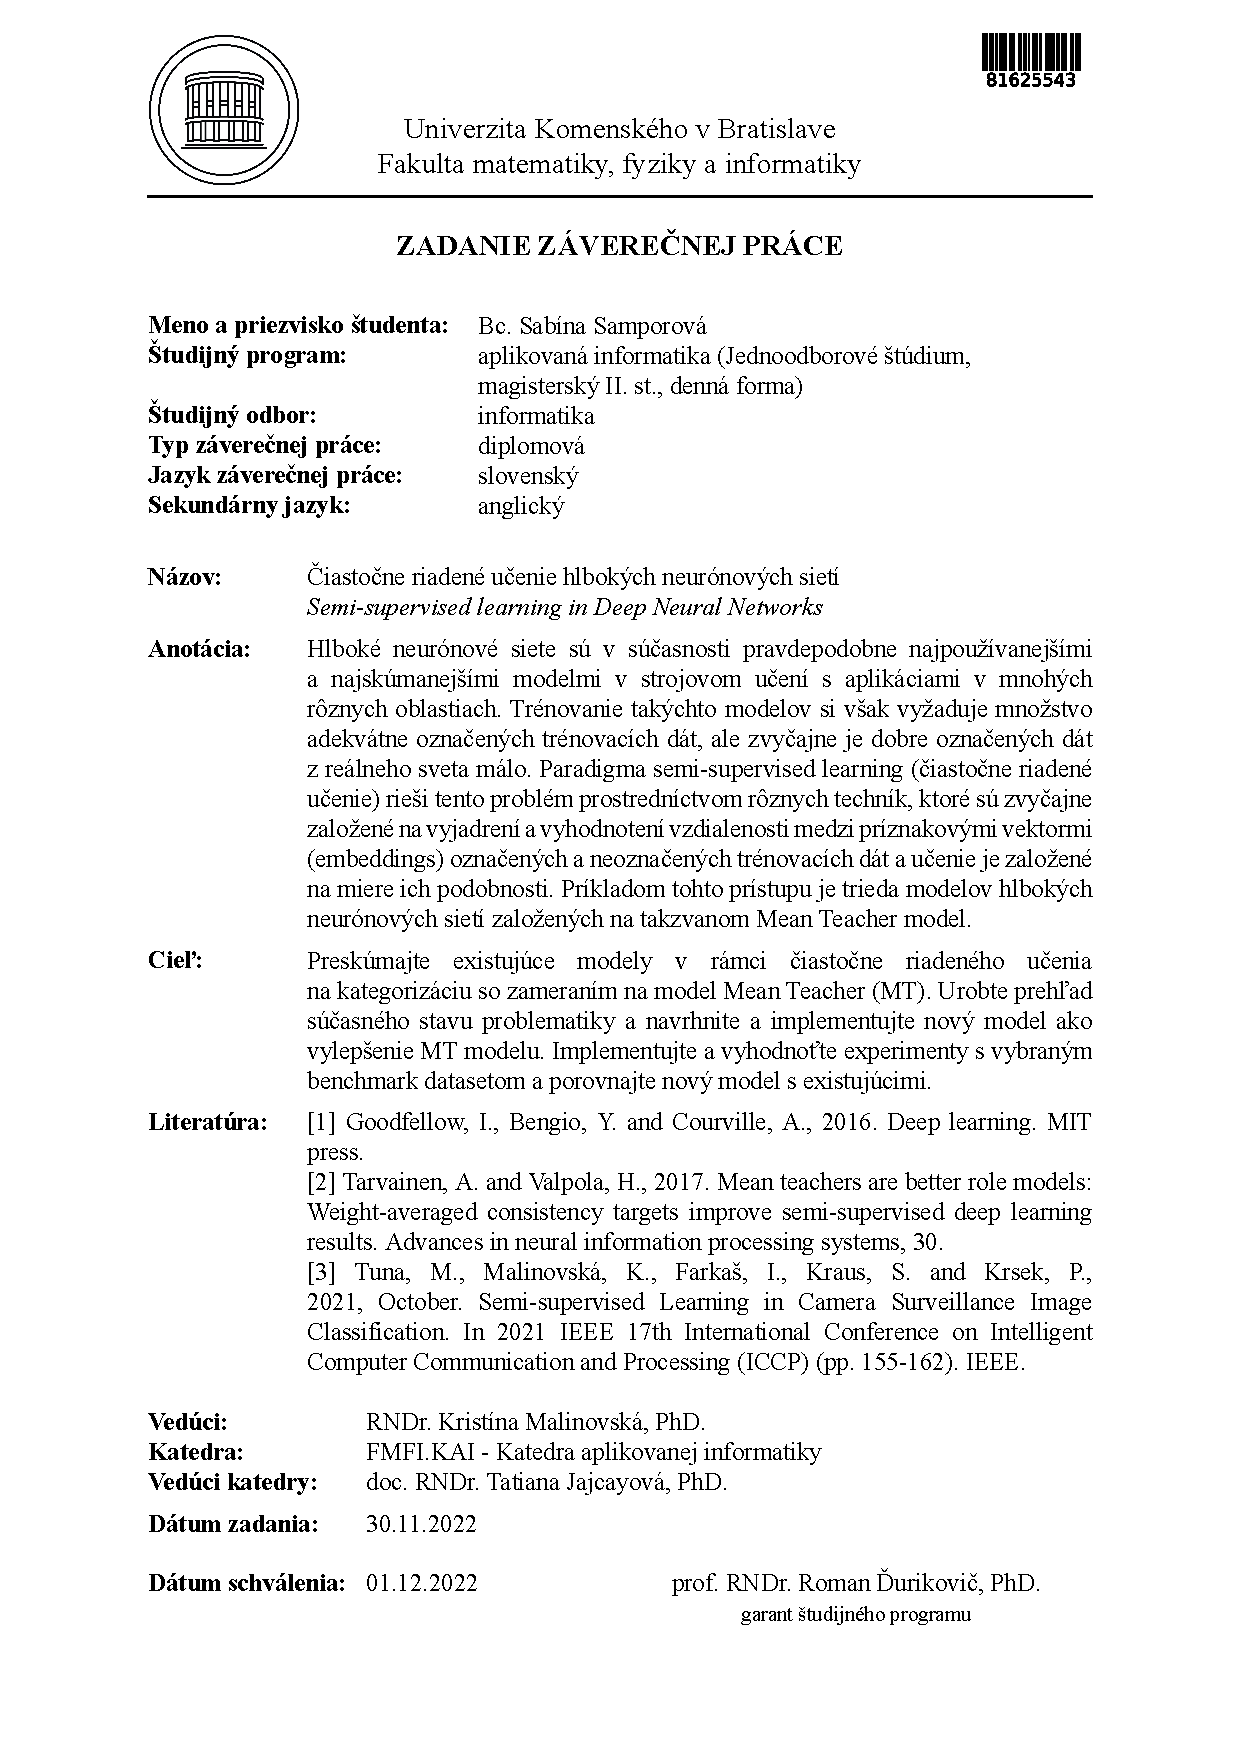
\includepdf{zadanie/zadanie.pdf}

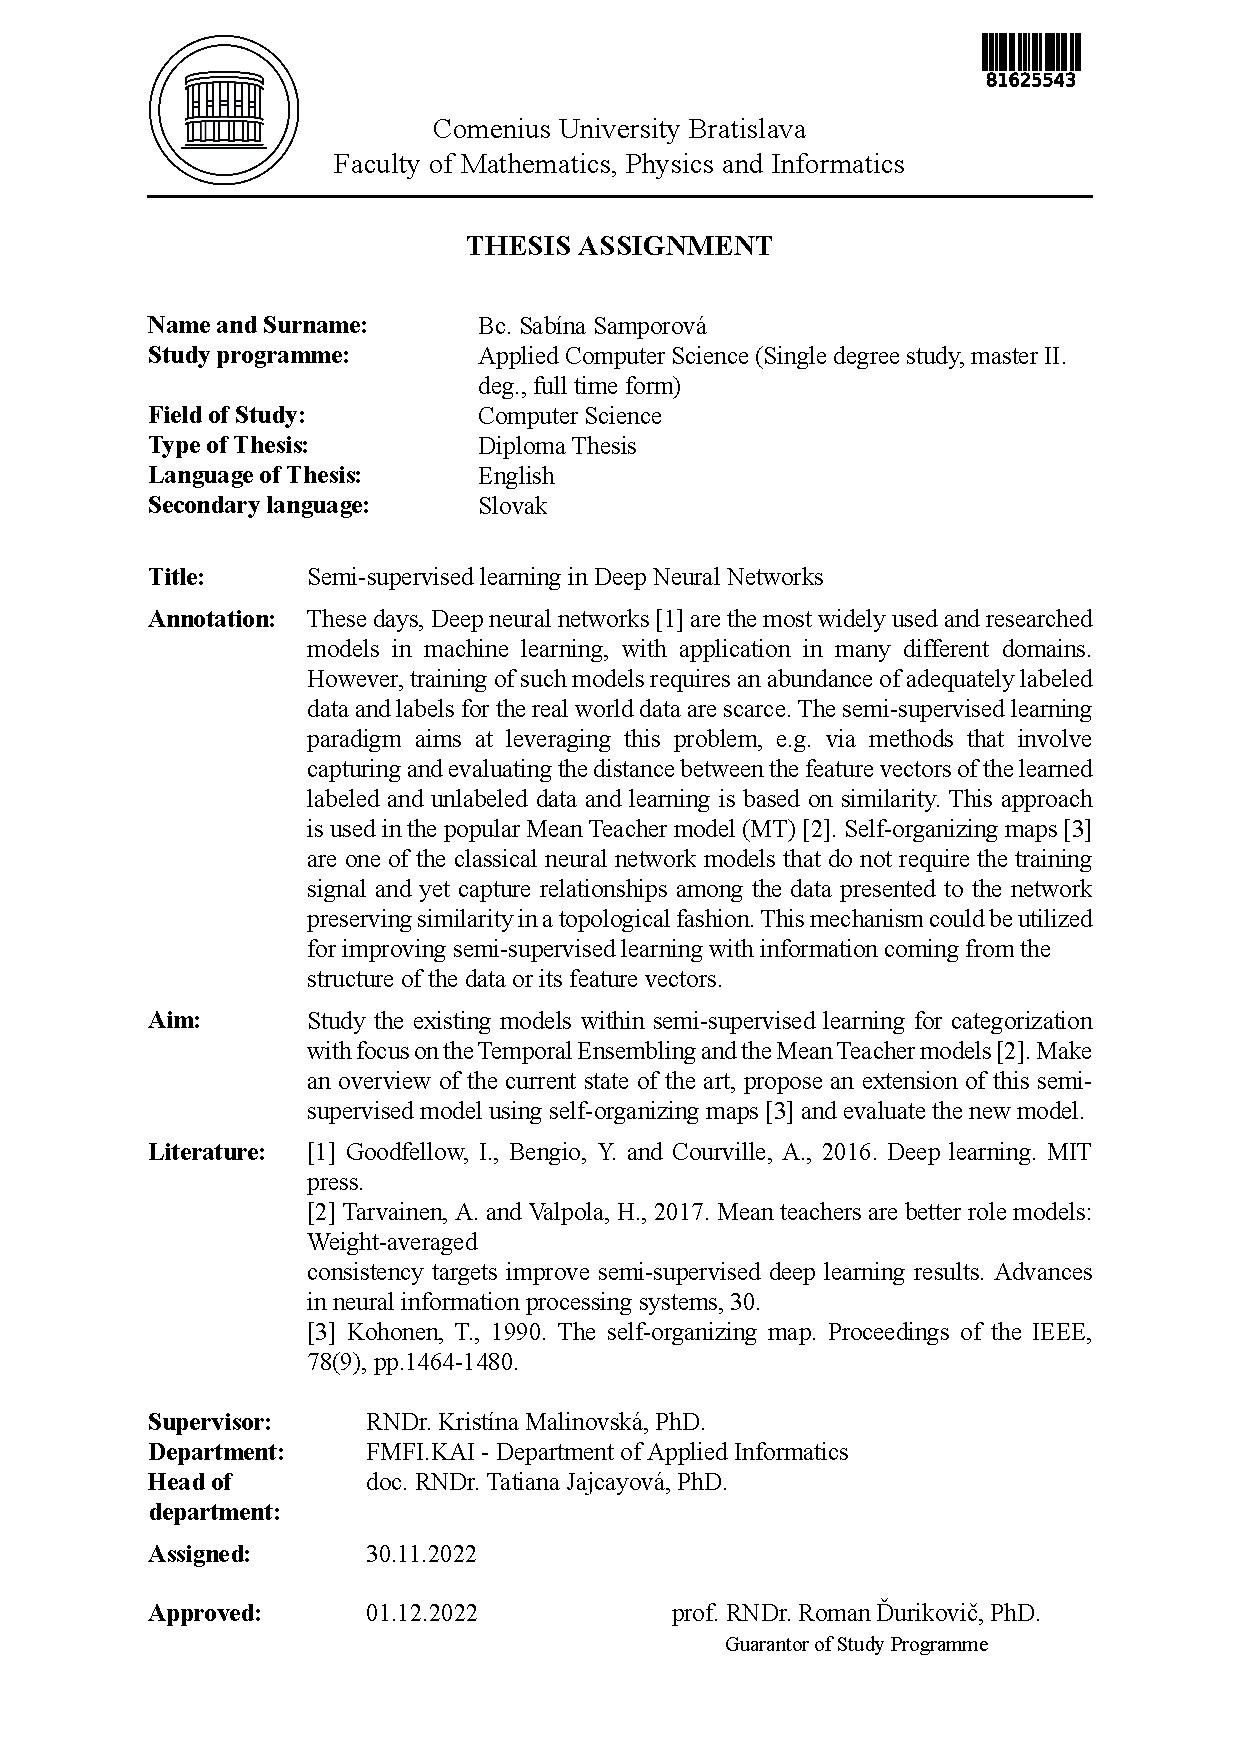
\includepdf{zadanie/zadanie-zp-en.pdf}

% --- Koniec zadania


% -------------------
%   Poďakovanie - nepovinné
% -------------------
\newpage
\pagestyle{plain}
~

\vfill
{\bf Acknowledgments:} % \color{red} TODO \color{black}


% --- Koniec poďakovania

% -------------------
%   Abstrakt - Slovensky
% -------------------
\newpage 
\section*{Abstrakt}

\color{red}
Hlboké neurónové siete sú v súčasnosti pravdepodobne najpoužívanejšími a najskúmanejšími modelmi v strojovom učení s aplikáciami v mnohých rôznych oblastiach. Trénovanie takýchto modelov si však vyžaduje množstvo adekvátne označených trénovacích dát, ale zvyčajne je dobre označených dát z reálneho sveta málo. Paradigma semi-supervised learning (čiastočne riadené učenie) rieši tento problém prostredníctvom rôznych techník, ktoré sú zvyčajne založené na vyjadrení a vyhodnotení vzdialenosti medzi príznakovými vektormi (embeddings) označených a neoznačených trénovacích dát a učenie je založené na miere ich podobnosti. Príkladom tohto prístupu je trieda modelov hlbokých neurónových sietí založených na takzvanom Mean Teacher model. V tejto práci skúmame spomínaný model a možnosti jeho vylepšenia s využitím samoorganizujúceho princípu.

\color{black}



\paragraph*{Kľúčové slová:} 


% --- Koniec Abstrakt - Slovensky


% -------------------
% --- Abstrakt - Anglicky 
% -------------------
\newpage 
\section*{Abstract}

\color{red}

These days, Deep neural networks are the most widely used and researched models in machine learning, with application in many different domains. However, training of such models requires an abundance of adequately labeled data and labels for the real world data are scarce. The semi-supervised learning paradigm aims at leveraging this problem via various different techniques that would typically involve capturing and evaluating the distance between the feature vectors of the learned labeled and unlabeled data and learning is based on similarity. This approach is used for example in the popular Mean Teacher model (MT). In this thesis, we investigate this model and look for posibilities of improvement using principle of self-organization.

\color{black}




\paragraph*{Keywords:} neural networks, semi-supervised learning, mean-teacher model, unsupervised learning, self-organizing map % , \color{red} TODO \color{black}


% --- Koniec Abstrakt - Anglicky

% -------------------
% --- Predhovor - v informatike sa zvacsa nepouziva
% -------------------
%\newpage 
%
%
%\chapter*{Preface} %
%
%Predhovor je všeobecná informácia o práci, obsahuje hlavnú charakteristiku práce 
%a okolnosti jej vzniku. Autor zdôvodní výber témy, stručne informuje o cieľoch 
%a význame práce, spomenie domáci a zahraničný kontext, komu je práca určená, 
%použité metódy, stav poznania; autor stručne charakterizuje svoj prístup a svoje
%hľadisko. 
%
% --- Koniec Predhovor


% -------------------
% --- Obsah
% -------------------

\newpage 

\tableofcontents

% ---  Koniec Obsahu

% -------------------
% --- Zoznamy tabuliek, obrázkov - nepovinne
% -------------------

\newpage 

\listoffigures
\listoftables

% ---  Koniec Zoznamov

\mainmatter
\pagestyle{headings}

\input 0-intro.tex 

\input 1-overview.tex

\input 2-bmt-exp.tex

\input 3-proposition.tex

\input 4-som-loss.tex

\input 5-som-fv-cifar.tex

\input 6-research-results.tex

\input 7-conclusion.tex

%\input kapitola.tex

%\input latex.tex



%\input zaver.tex

% -------------------
% --- Bibliografia
% -------------------


\newpage	

\backmatter

\thispagestyle{empty}
\clearpage

\bibliographystyle{plain}
\bibliography{literatura} 

%Prípadne môžete napísať literatúru priamo tu
%\begin{thebibliography}{5}
 
%\bibitem{br1} MOLINA H. G. - ULLMAN J. D. - WIDOM J., 2002, Database Systems, Upper Saddle River : Prentice-Hall, 2002, 1119 s., Pearson International edition, 0-13-098043-9

%\bibitem{br2} MOLINA H. G. - ULLMAN J. D. - WIDOM J., 2000 , Databasse System implementation, New Jersey : Prentice-Hall, 2000, 653s., ???

%\bibitem{br3} ULLMAN J. D. - WIDOM J., 1997, A First Course in Database Systems, New Jersey : Prentice-Hall, 1997, 470s., 

%\bibitem{br4} PREFUSE, 2007, The Prefuse visualization toolkit,  [online] Dostupné na internete: <http://prefuse.org/>

%\bibitem{br5} PREFUSE Forum, Sourceforge - Prefuse Forum,  [online] Dostupné na internete: <http://sourceforge.net/projects/prefuse/>

%\end{thebibliography}

%---koniec Referencii

% -------------------
%--- Prilohy---
% -------------------

%Nepovinná časť prílohy obsahuje materiály, ktoré neboli zaradené priamo  do textu. Každá príloha sa začína na novej strane.
%Zoznam príloh je súčasťou obsahu.
%
%\input appendixA.tex

%\input appendixB.tex

\end{document}






